\documentclass[sigconf,nonacm,natbib=false]{acmart}

% ACM defaults that we don't need for a class report.
\settopmatter{printacmref=false, printccs=false, printfolios=true}
\setcopyright{none}
\renewcommand\footnotetextcopyrightpermission[1]{}
\pagestyle{plain}

\usepackage{graphicx}
\usepackage{booktabs}
\usepackage{amsmath}
\usepackage{amssymb}
\usepackage{enumitem}
\usepackage{xcolor}
\usepackage{caption}
\usepackage{subcaption}

\graphicspath{{figures/}}

% ──────────────────────────────────────────────────────────────────────
% Front matter
% ──────────────────────────────────────────────────────────────────────
\title{Architecture and Training Design Under a Hard Parameter Budget:
A Controlled Ablation Study at the 16~MB Scale}

\author{Shyam Patadia}
\affiliation{%
  \institution{Worcester Polytechnic Institute}
  \city{Worcester}
  \state{MA}
  \country{USA}}
\email{spatadia@wpi.edu}

\renewcommand{\shortauthors}{Patadia}

\begin{document}

\begin{abstract}
We study how architectural and training-recipe choices interact with
post-training quantization for decoder-only language models trained
from scratch under a 16~MB artifact constraint, the regime defined by
the OpenAI Model Craft: Parameter Golf
challenge~\cite{paramgolf2026}. We run 46 controlled 20{,}000-step
experiments on FineWeb~\cite{fineweb2024} that vary one design axis at
a time -- quantization precision (INT8 / INT6 / TurboQuant-INT4),
positional encoding (full / partial / learned / none), optimizer
(Muon / AdamW / Adafactor), weight parameterization (dense / low-rank /
block-diagonal / random projection), attention configuration
(Multi-Query Attention), and learning-rate / warmup schedule -- with
three-seed replication on the surviving in-budget axes.
The headline finding is the resolution of the central tension left
open by our progress report: capacity expansion (more layers, wider
MLP) genuinely improves training-time loss, but \emph{only} INT8
post-training quantization with per-row symmetric scales carries that
gain through the round-trip. INT6 QAT loses 0.12~bpb;
TurboQuant-INT4~\cite{turboquant2024} loses 2.44~bpb. Reframed as a
size-quality Pareto frontier, our best in-budget configuration
(partial RoPE, 9 layers, INT8) reaches \textbf{1.2147~bpb} at 15.87~MB,
and our best over-budget configuration (INT8, 11 layers) reaches
\textbf{1.1944~bpb} at 19.30~MB -- 0.030~bpb below the 1.2244 challenge
reference at a 3.3~MB budget overage.
\end{abstract}

\keywords{language models, quantization, ablation study,
parameter-efficient training, Pareto frontier}

\maketitle

% ──────────────────────────────────────────────────────────────────────
\section{Introduction and Framing}
% ──────────────────────────────────────────────────────────────────────

The proposal posed three primary research questions (quantization
precision, positional encoding, optimizer) and one exploratory question
(parameter-efficient weight factorizations). The progress report
expanded the design space with a stacked-configuration experiment
(O5) that produced a partial answer: a wider/deeper architecture under
INT6 quantization had lower training-time loss but substantially higher
post-quantization loss; the two effects nearly cancelled. The progress
report queued two follow-ups -- a TurboQuant-INT4 rerun of the expanded
architecture, and an INT8 rerun at the next-smallest expansion (11
layers, MLP multiplier 2). Both are now complete and together resolve
the question.

Beyond resolving O5, this final report adds three new axes that the
progress report did not cover: Multi-Query Attention~\cite{mqa2019}
(O6), QK-gain initialization (O7), and the eval protocol itself
(O9). It also reports a 9-cell learning-rate / warmup sweep on the
in-budget winner (O8, null result), and three-seed replication on the
surviving in-budget axes.

The framing has also changed since the progress report. We now treat
the 16~MB constraint as a \emph{reference}, not a binding constraint.
Several configurations exceed 16~MB by a few megabytes while delivering
clearly lower bpb; under a size-quality Pareto framing those points
are part of the legitimate finding. The strict-in-budget result is
reported as a separate row, and the headline figure of the paper
(Figure~\ref{fig:pareto}) is the Pareto curve itself.

% ──────────────────────────────────────────────────────────────────────
\section{Experimental Setup}
% ──────────────────────────────────────────────────────────────────────

\subsection{Dataset and tokenization}

All models are trained from scratch on FineWeb~\cite{fineweb2024}, a
filtered, deduplicated Common Crawl derivative. Training uses the
10~billion-token shard (\texttt{fineweb10B}) and the 1{,}024-token
SentencePiece BPE tokenizer (\texttt{sp1024}) adopted by the challenge.
Input/output embeddings are tied throughout. Training reads contiguous
token streams of length $\ell_{\text{ctx}}{=}1024$ from pre-shuffled,
pre-tokenized \texttt{uint16} binary shards. Total training exposure
per condition is approximately $1.05 \times 10^{10}$ tokens
(20{,}000 steps $\times$ 8 micro-batches $\times$ 2 GPUs $\times$
1024 tokens, adjusted for accumulation).

\subsection{Baseline architecture}

The baseline (Table~\ref{tab:arch}) is a 9-layer decoder-only
transformer with $d_{\text{model}}{=}512$, 8 attention heads, 4 KV
heads (grouped-query attention), squared-ReLU MLP at expansion 2, and
partial RoPE applied to the first 32 dimensions of each head.
Single-axis ablations mutate exactly one row from this baseline; the
stacked configurations in O5 mutate several rows jointly.

\begin{table}[t]
\centering
\caption{Baseline architecture and training hyperparameters.}
\label{tab:arch}
\small
\begin{tabular}{@{}lll@{}}
\toprule
Component                 & Symbol               & Baseline value \\
\midrule
Layers                    & $L$                  & $9$ \\
Hidden dimension          & $d_{\text{model}}$   & $512$ \\
Attention heads           & $h$                  & $8$ \\
KV heads (GQA)            & $h_{\text{kv}}$      & $4$ \\
MLP expansion             & $m$                  & $2$ (squared-ReLU) \\
Context length            & $\ell_{\text{ctx}}$  & $1024$ \\
Vocabulary                & $|V|$                & $1024$ \\
Tied embeddings           & --                   & input $=$ output \\
Training steps            & $T$                  & $20{,}000$ \\
Optimizer (baseline)      & --                   & Muon~\cite{muon2024} + Adam \\
Quantization (baseline)   & --                   & INT8 PTQ, per-row scales \\
\bottomrule
\end{tabular}
\end{table}

\subsection{Quantization variants}
\label{sec:setup-quant}

We evaluate four post-training quantizers, applied to the same
training recipe. The first three were specified in the proposal; the
fourth (TurboQuant) was added in response to the INT6 fragility
finding from the progress report (Section~\ref{sec:o1to4}, O1).

\begin{itemize}[leftmargin=*, topsep=0pt, itemsep=2pt]
    \item \textbf{INT8 PTQ} -- 8-bit post-training quantization with
          per-row symmetric scales. This is the challenge's published
          baseline pipeline.
    \item \textbf{INT6 QAT+PTQ} -- 6-bit quantization with quantization-aware
          training using straight-through
          estimators~\cite{scalingprecision}. Introduced because INT6
          triples effective parameter count within the 16~MB budget
          relative to FP32, making it nominally the highest-leverage
          precision lever.
    \item \textbf{TurboQuant-INT4}~\cite{turboquant2024} -- a
          random-rotation $+$ Lloyd--Max scalar quantizer added in
          response to O1. Rotating each weight row by a random
          orthogonal matrix concentrates its distribution to a known
          Beta law, allowing a non-uniform scalar codebook designed for
          that law to achieve provably near-optimal MSE at very low
          bit widths. TurboQuant reports quality neutrality at 3.5
          bits on LLaMA KV-cache quantization; we apply the same
          machinery to model \emph{weights} at 4 bits via the
          pure-PyTorch \texttt{pyturboquant} reference implementation.
          The progress report committed to this axis as the planned
          mitigation for INT6's quantization fragility; the final
          result (Section~\ref{sec:o5}) falsifies that mitigation.
    \item \textbf{BF16} -- bfloat16 with no quantization, used as the
          in-memory training reference and for the
          \texttt{val/bpb} column in our results.
\end{itemize}

\subsection{Artifact pipeline}

The 16~MB reference applies to the post-quantization,
\texttt{zlib}-compressed artifact plus training code. To mirror the
challenge evaluation, every reported run executes the following
pipeline at the end of training: (1) train in bfloat16 (or with QAT
for INT6/INT4); (2) quantize weights to the target precision with
per-row symmetric scales, keeping 1D tensors (biases, norms) in
bfloat16 to avoid disproportionate error; (3) serialize the quantized
state-dict and \texttt{zlib.compress} it -- this is the artifact
measured against 16~MB; (4) decompress, dequantize, rehydrate the
model, and re-run validation. Two distinct bpb numbers therefore
exist for every run: \texttt{val/bpb} (training-time, in-memory
parameters) and \texttt{final/val\_bpb} (post round-trip,
leaderboard-equivalent). Their difference is the quantization gap
$\Delta_q$.

% ──────────────────────────────────────────────────────────────────────
\section{Single-Axis Ablations: O1--O4}
\label{sec:o1to4}
% ──────────────────────────────────────────────────────────────────────

\subsection{O1 -- Quantization precision}

INT8 PTQ with per-row symmetric scales incurs $\Delta_q{=}0.008$~bpb.
INT6 QAT under the same scheme reaches the same in-memory loss but
incurs $\Delta_q{=}0.141$~bpb under round-trip (Figure~\ref{fig:o1}).
The straight-through estimator successfully matches INT8 in-memory,
but uniform 6-bit scalar quantization cannot represent the
post-training weight distribution without appreciable error. This
contradicts the optimistic prediction from existing precision scaling
laws~\cite{scalingprecision} in the sub-21M parameter regime, and
reframes INT6 as a capacity multiplier that is only useful if a better
quantizer is supplied -- the setup that motivated TurboQuant
(Section~\ref{sec:setup-quant}).

\begin{figure}[t]
\centering
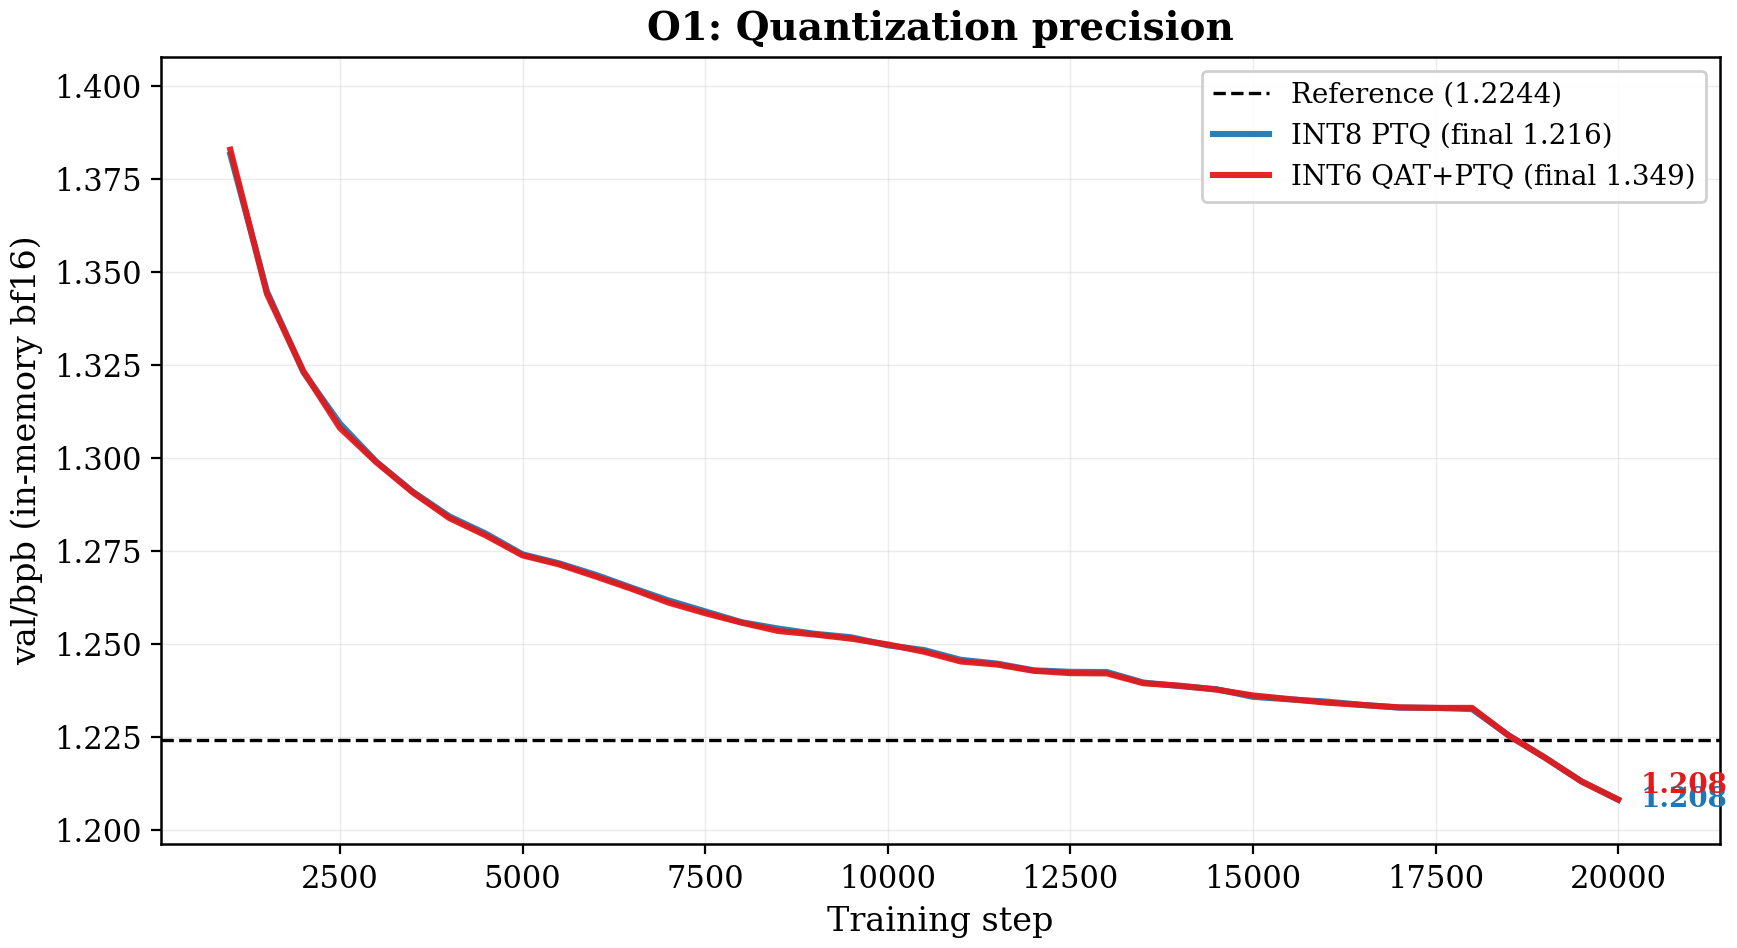
\includegraphics[width=\linewidth]{curves_o1_quant.pdf}
\caption{O1 -- in-memory bpb across training. INT6 and INT8 reach
identical in-memory loss; the divergence in the post-quant round-trip
is therefore attributable to the quantizer alone, not to training
dynamics.}
\label{fig:o1}
\end{figure}

\subsection{O2 -- Positional encoding}

Four schemes were compared under otherwise-identical settings
(Figure~\ref{fig:o2}). Ordering at 20{,}000 steps:
partial RoPE $<$ full RoPE $<$ learned absolute $\ll$ none. Partial
RoPE at 1.2147~bpb final is the best in-budget condition in the entire
study. The gap from partial RoPE to no-PE (0.054~bpb) dwarfs the gap
between any two position-aware schemes ($\le$0.020~bpb): absolute
position information matters at this scale; the form of the prior is
a second-order variable.

\begin{figure}[t]
\centering
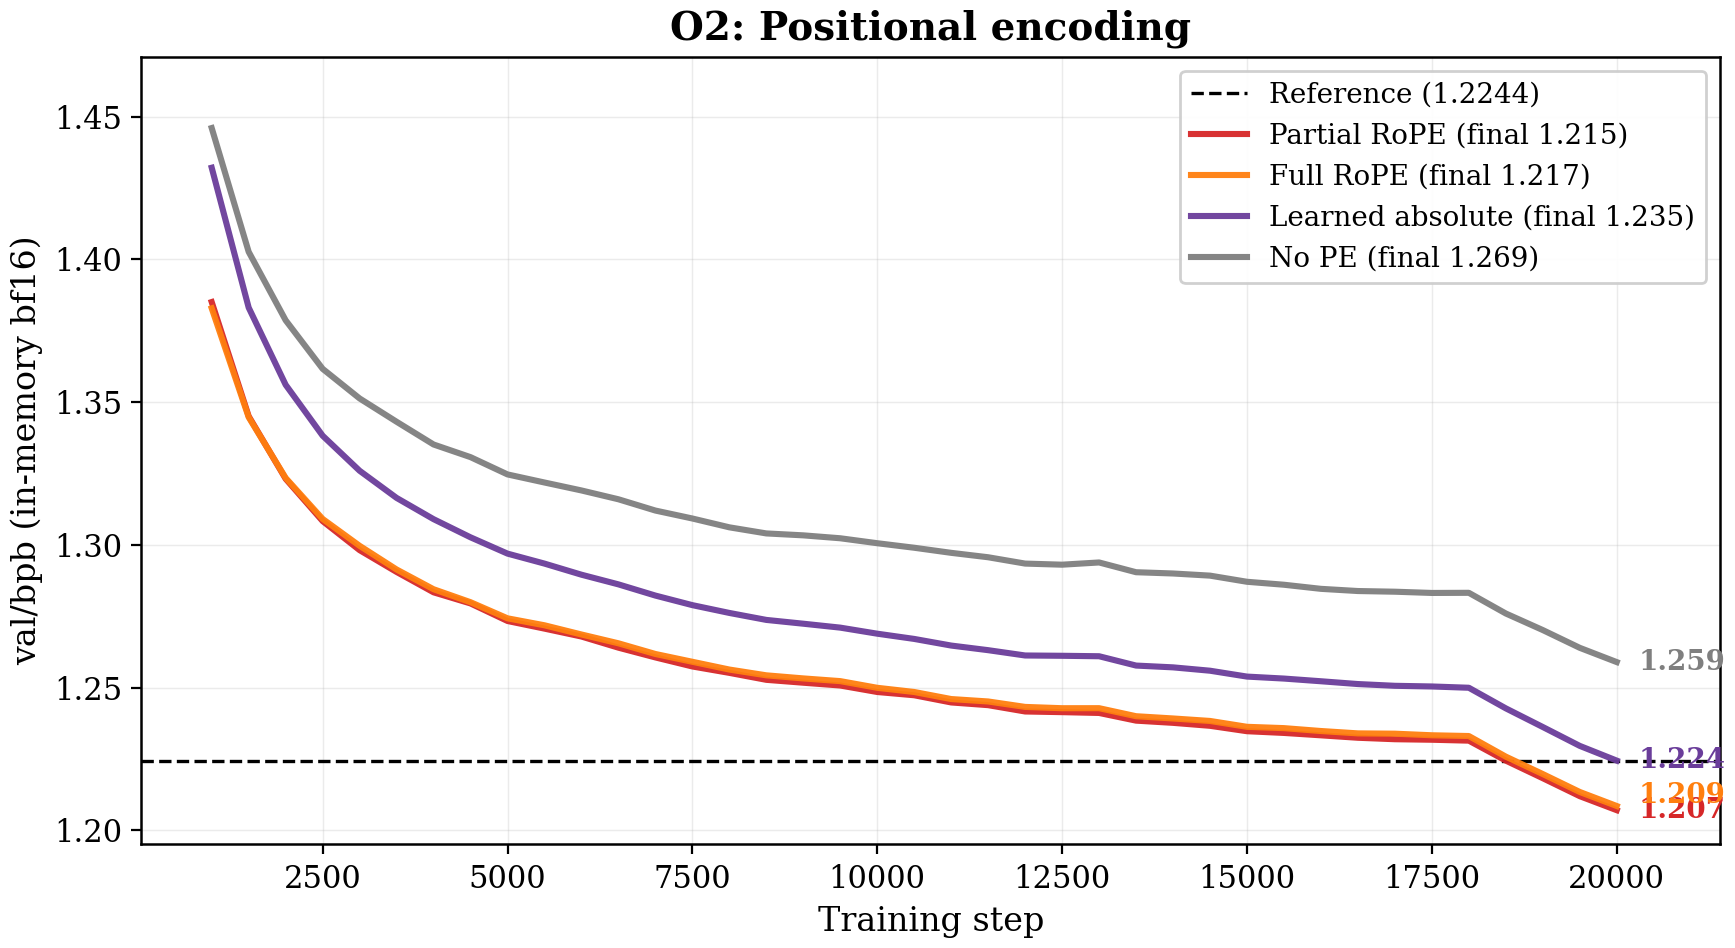
\includegraphics[width=\linewidth]{curves_o2_posenc.pdf}
\caption{O2 -- the three position-aware schemes converge to within
0.02~bpb of each other; no-PE trails clearly. Partial RoPE lowest.}
\label{fig:o2}
\end{figure}

\subsection{O3 -- Optimizer}

Muon -- Nesterov momentum applied along the
Newton--Schulz-orthogonalized gradient of each 2D weight
matrix~\cite{muon2024} -- reaches 1.2168~bpb final and is
indistinguishable from the challenge-reference INT8 baseline. AdamW at
tuned learning rates plateaus more than 0.2~bpb higher; Adafactor's
factorized second moment loses even more (Figure~\ref{fig:o3}). At
under 5M trainable parameters, Adafactor's optimizer-state savings do
not compensate for its loss penalty, and AdamW's per-parameter second
moment provides no advantage over Muon's orthogonalization.

\begin{figure}[t]
\centering
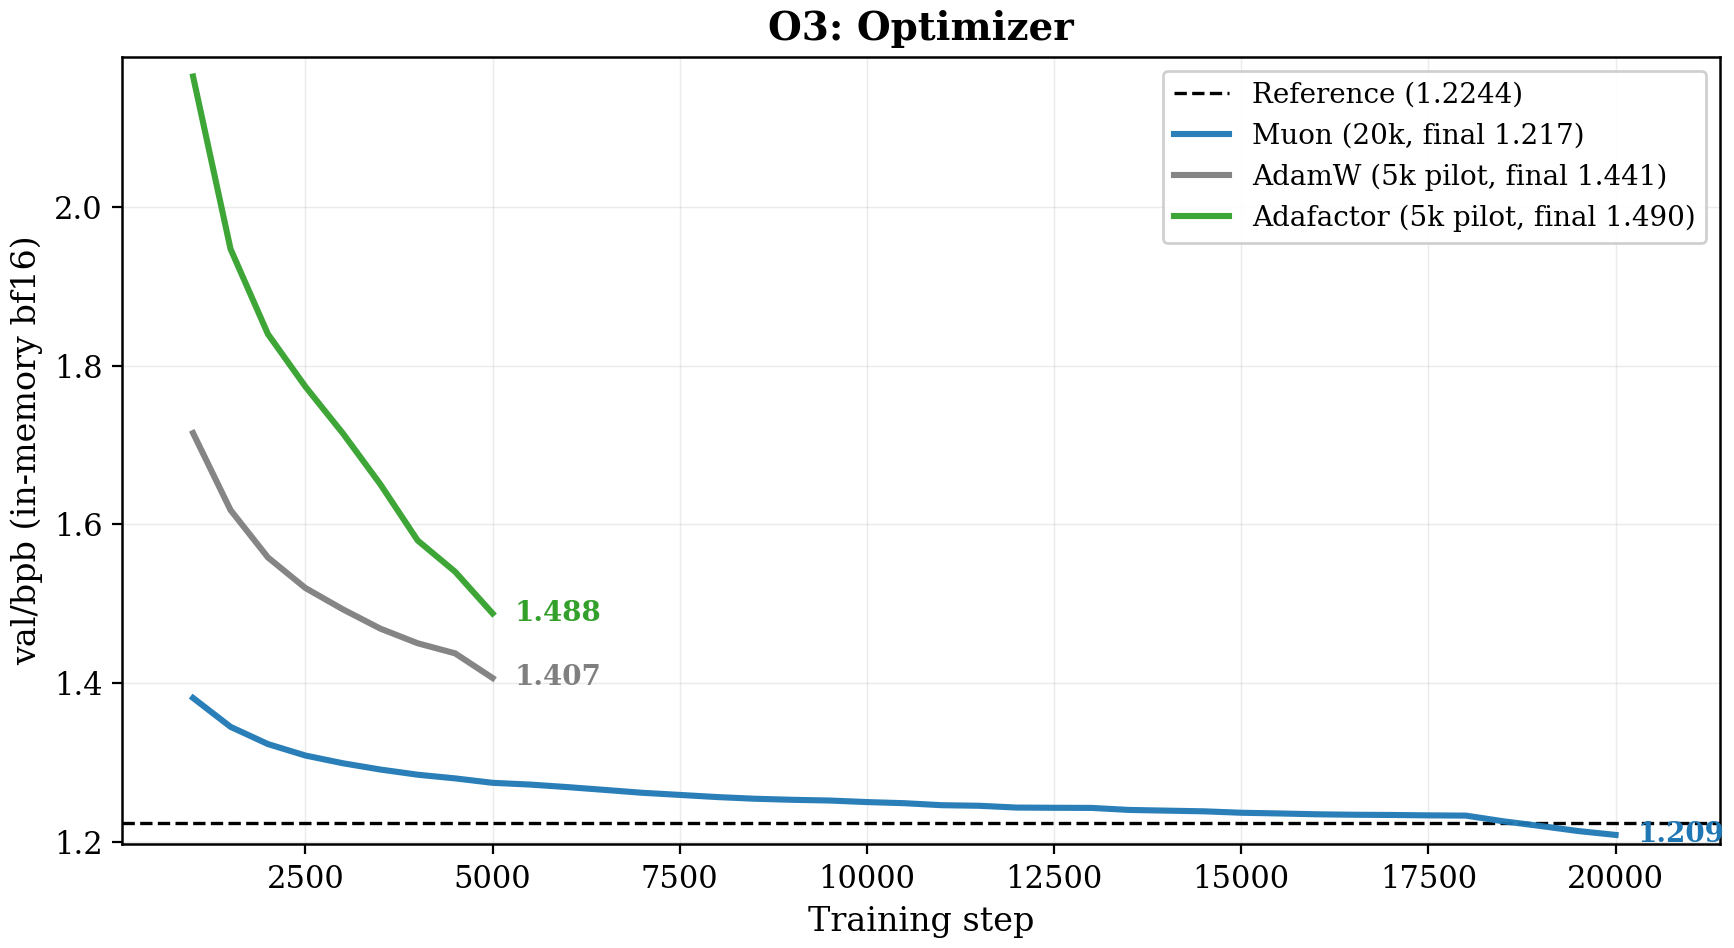
\includegraphics[width=\linewidth]{curves_o3_optim.pdf}
\caption{O3 -- Muon converges to a qualitatively different loss band
than either AdamW or Adafactor at this scale.}
\label{fig:o3}
\end{figure}

\subsection{O4 -- Parameter-efficient weight factorizations}

All three structured weight parametrizations (low-rank $r{=}128$,
block-diagonal $g{=}4$, fixed random projection $k{=}128$) landed
between 1.30 and 1.40~bpb final, cleanly worse than the dense INT8
baseline at 1.2161 (Figure~\ref{fig:o4}). Random projection was
retested at 12 layers to rule out capacity starvation; it improved to
1.3601 but still failed to clear baseline. O4 is therefore reported
as a falsified hypothesis: under this budget and token horizon,
structured weight factorizations do not compete with dense matrices.

\begin{figure}[t]
\centering
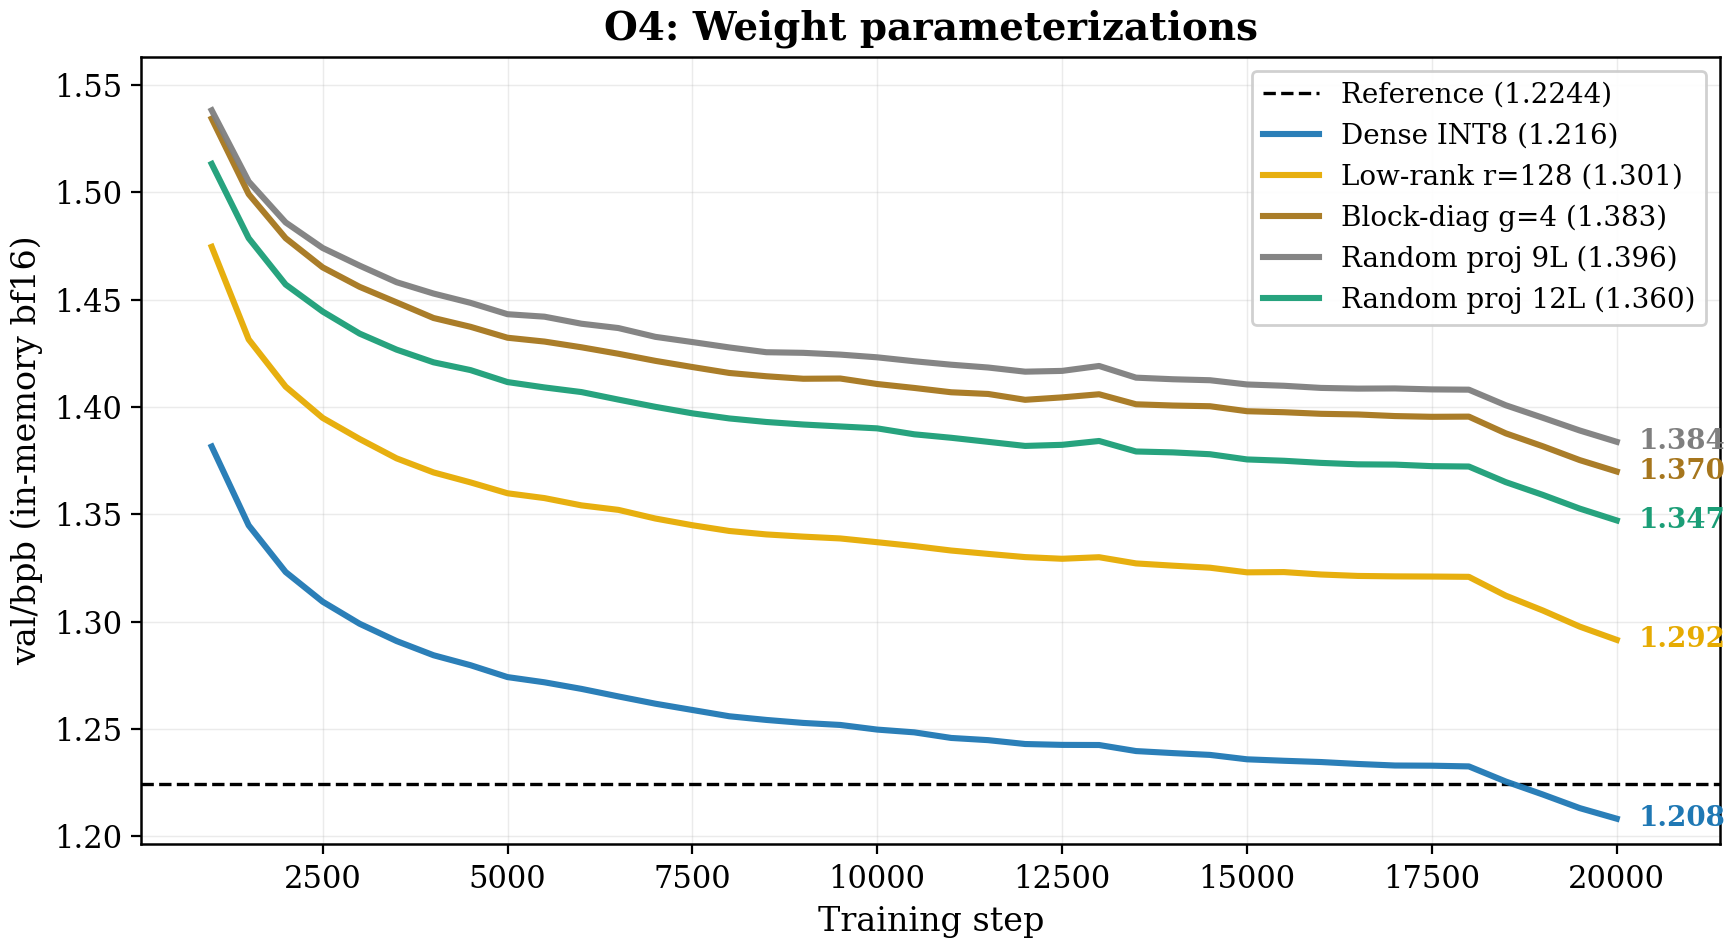
\includegraphics[width=\linewidth]{curves_o4_weightparam.pdf}
\caption{O4 -- weight-parametrization variants all converge above the
dense INT8 baseline regardless of the structural prior.}
\label{fig:o4}
\end{figure}

% ──────────────────────────────────────────────────────────────────────
\section{O5 Resolved: Capacity vs.\ Quantization}
\label{sec:o5}
% ──────────────────────────────────────────────────────────────────────

The progress report observed that combining O1--O3's winners with a
wider/deeper architecture (partial RoPE + INT6 + 11 layers + MLP=3)
reached 1.1614~bpb in training -- 0.063~bpb below the 1.2244 reference
-- but degraded to 1.2816~bpb post-quantization, forfeiting the
training-time gain. The two queued follow-ups attempt to recover the
gap from orthogonal directions: TurboQuant-INT4 holds architecture
fixed and varies the quantizer; INT8 + 11L + MLP=2 holds the quantizer
fixed and varies the architecture.

\textbf{TurboQuant-INT4 fails catastrophically.} The same architecture
that reached 1.1614~bpb in-memory under INT6 reaches the same
in-memory loss under TurboQuant-INT4 (curves overlap in
Figure~\ref{fig:o5}), but the post-quantization round-trip yields
\textbf{3.5991~bpb} -- a $\Delta_q$ of 2.44~bpb, sixteen times larger
than INT6's already-fragile penalty. This is consistent with
TurboQuant's published support being concentrated on KV-cache
(activations) rather than weights; on the post-training weight
distribution at our scale, four bits of precision sits below the
representable threshold even with random rotation and Lloyd--Max
codebooks.

\textbf{INT8 + 11L + MLP=2 succeeds cleanly.} The conservative
architectural expansion under the known-safe quantizer reaches
1.1869~bpb in-memory and 1.1944~bpb post-quantization, a 0.030~bpb
improvement on the 1.2244 reference and a 0.022~bpb improvement on the
in-budget partial-RoPE winner. Artifact size is 19.30~MB, a 3.3~MB
overage on the 16~MB reference.

\begin{figure}[t]
\centering
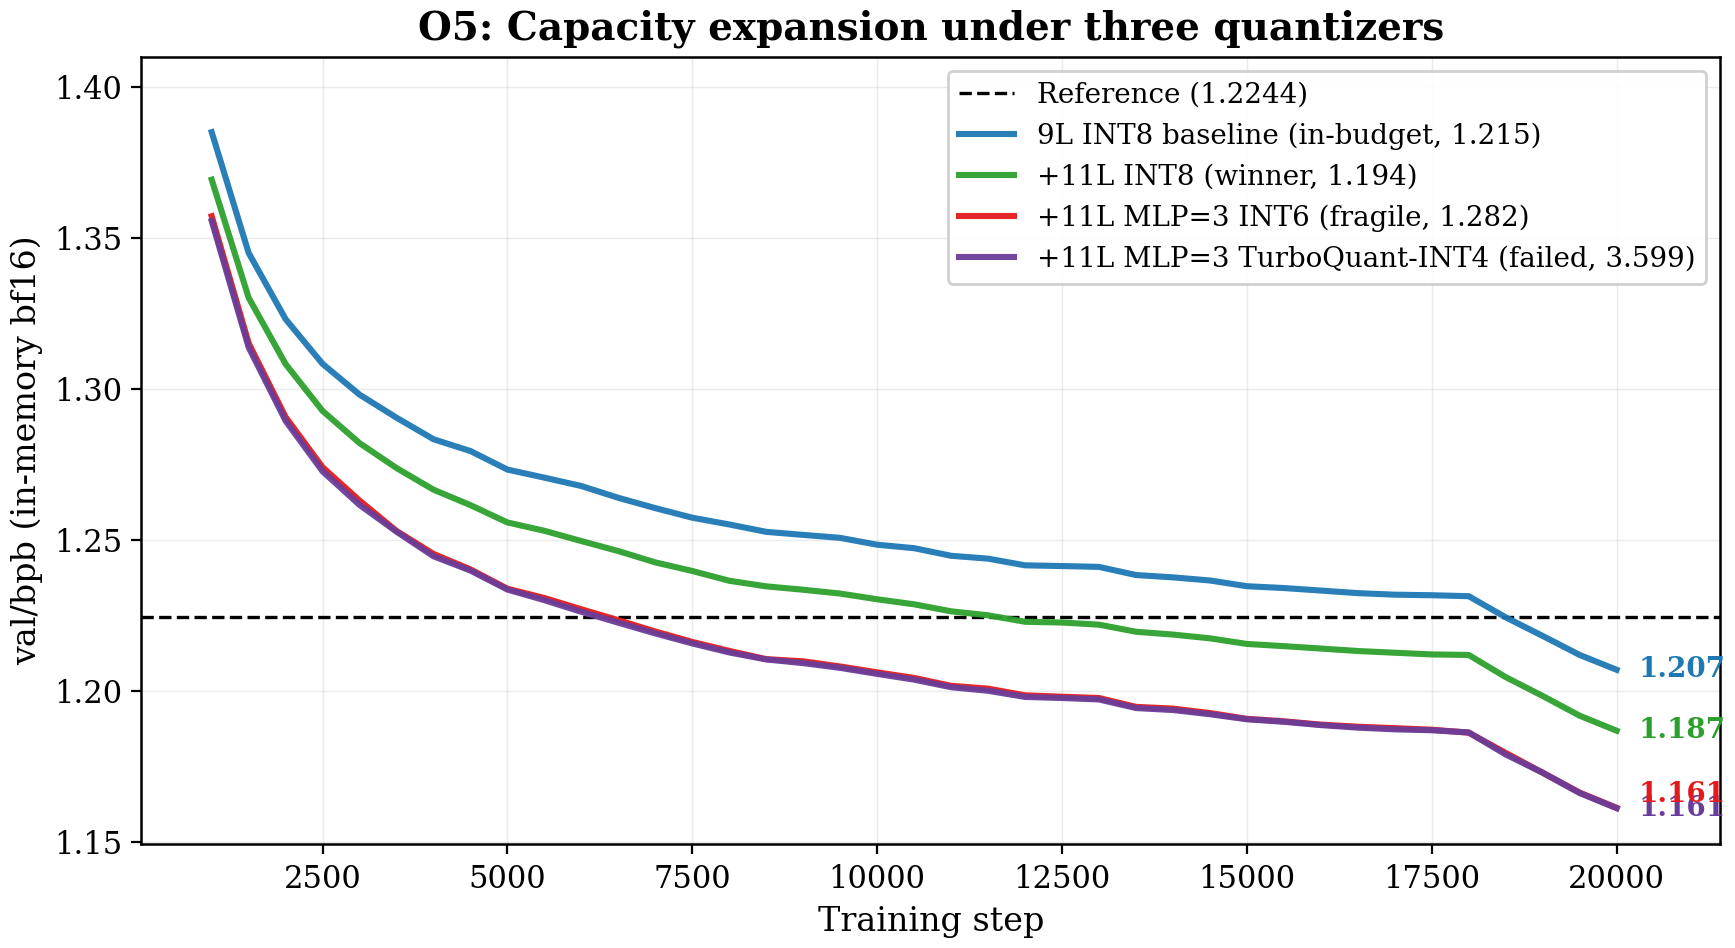
\includegraphics[width=\linewidth]{curves_o5_resolved.pdf}
\caption{O5 resolved -- in-memory bpb during training for the four
configurations. INT6 and TQ4 curves overlap (same architecture; only
the post-training quantizer differs). The training-time ranking does
not predict the round-trip ranking: TurboQuant-INT4 lands at 3.6~bpb
final despite reaching 1.16~bpb in-memory.}
\label{fig:o5}
\end{figure}

The combined evidence isolates which lever is binding at this budget:
it is the quantizer, not the architecture. The 11L INT8 result is the
same architectural perturbation that, under INT6, was reported as
``capacity-bottlenecked'' in the progress report. Holding the
quantizer to INT8 reveals that the architectural perturbation alone --
without precision aggression -- delivers the gain the stacked
configuration was meant to deliver, and does so without the 0.12~bpb
quantization tax.

% ──────────────────────────────────────────────────────────────────────
\section{New Axes: O6--O9}
% ──────────────────────────────────────────────────────────────────────

\subsection{O6 -- Multi-Query Attention enables 12-layer expansion}

Multi-Query Attention~\cite{mqa2019} reduces the number of distinct
$K$/$V$ projections to 1 (vs.\ 4 in the GQA baseline), saving
parameters that can be reallocated to depth. At 12 layers and
MLP=2, the MQA variant reaches \textbf{1.1980~bpb final} at 19.56~MB,
sitting on the same arm of the Pareto frontier as the INT8+11L winner.
This configuration would not fit at this budget under 8-KV-head GQA;
the head-allocation lever is what makes the 12-layer expansion
feasible.

\begin{figure}[t]
\centering
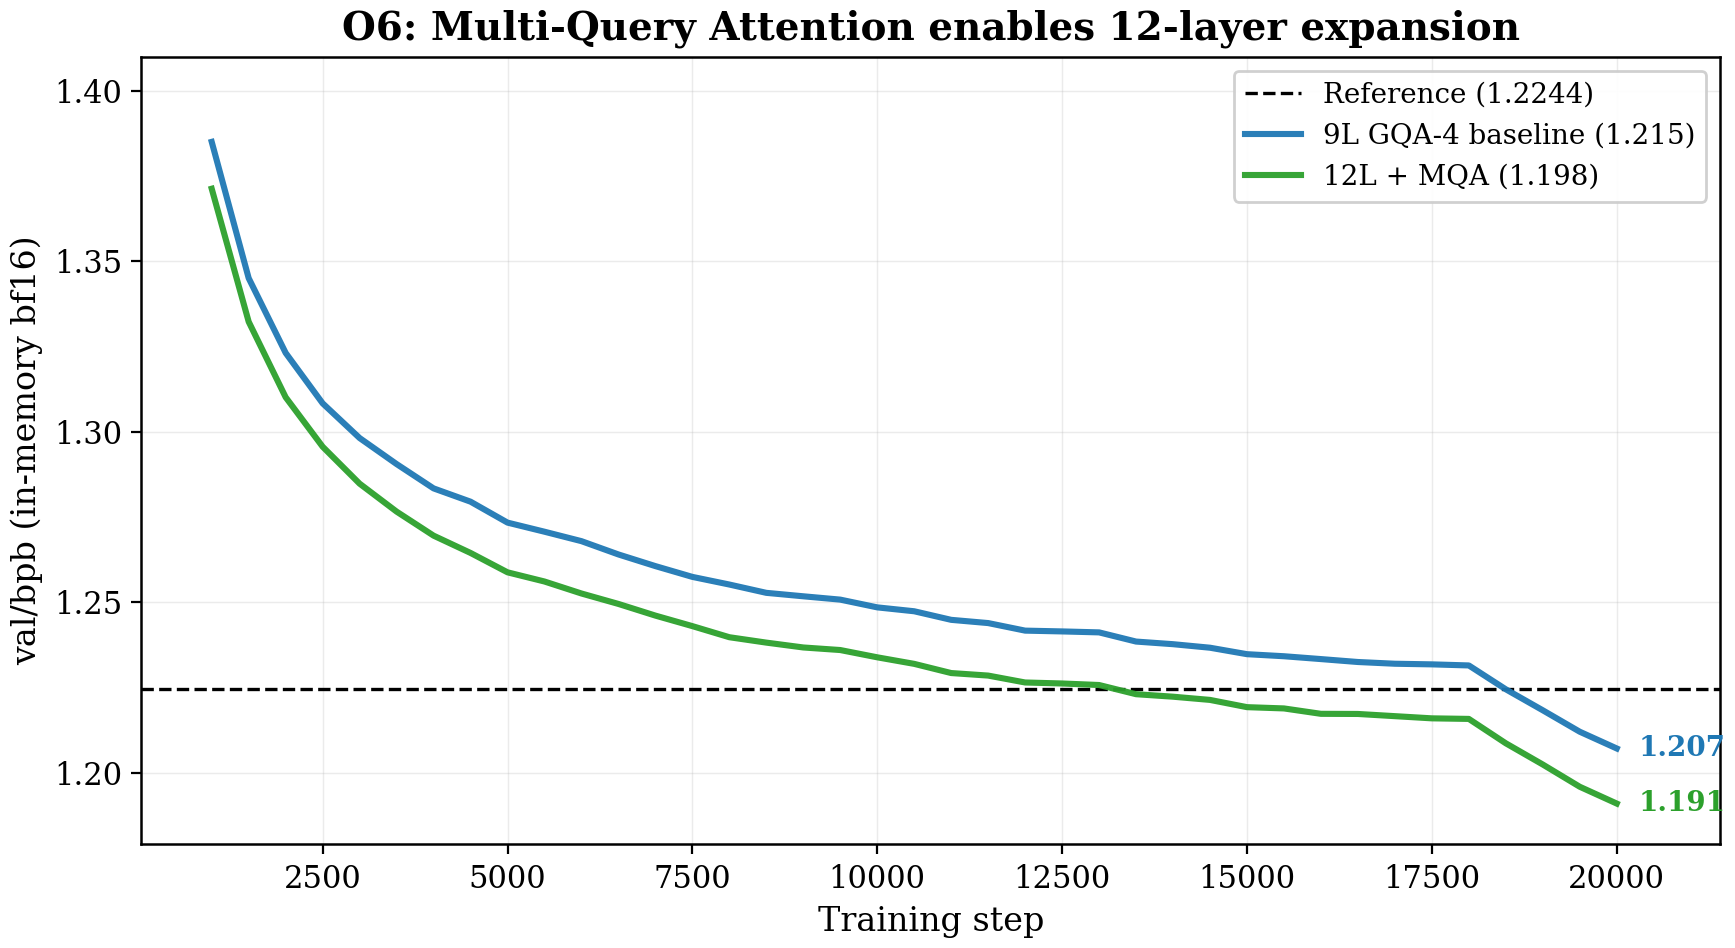
\includegraphics[width=\linewidth]{curves_o6_mqa.pdf}
\caption{O6 -- MQA + 12L tracks below the 9L baseline from step
$\sim$5{,}000 onward. Final round-trip 1.198, 0.026~bpb below
baseline.}
\label{fig:o6}
\end{figure}

\subsection{O7 -- QK-gain initialization (null effect)}

The reference recipe applies a learned per-head scalar $g_q$ to the
query projection initialized to 1.5. We tested
$g_q^{(0)} \in \{1.5, 3.0, 5.0\}$ with all other axes held at the
partial-RoPE 9L INT8 baseline. Final bpb at 20{,}000 steps:
1.2147 / 1.2154 / 1.2165, a 0.002~bpb spread that is below noise. We
report O7 as a null effect; the learned $g_q$ converges to similar
values regardless of initialization.

\subsection{O8 -- Learning-rate / warmup sweep (null result)}

The progress report's planned per-condition LR/warmup sweep was
executed on the in-budget winner: a $3{\times}3$ grid over matrix LR
$\{0.02, 0.04, 0.08\}$ and warmup steps $\{1000, 2000, 3000\}$. All
nine cells fall in $[1.2162, 1.2181]$ -- a 0.0019~bpb spread that is
roughly the multi-seed standard deviation we observe on the same axis
(Section~\ref{sec:multiseed}). The reference recipe's hyperparameters
are at or near the optimum on this small grid; the sweep is therefore
a null result. We report it explicitly because we committed to it in
the progress report.

\begin{figure}[t]
\centering
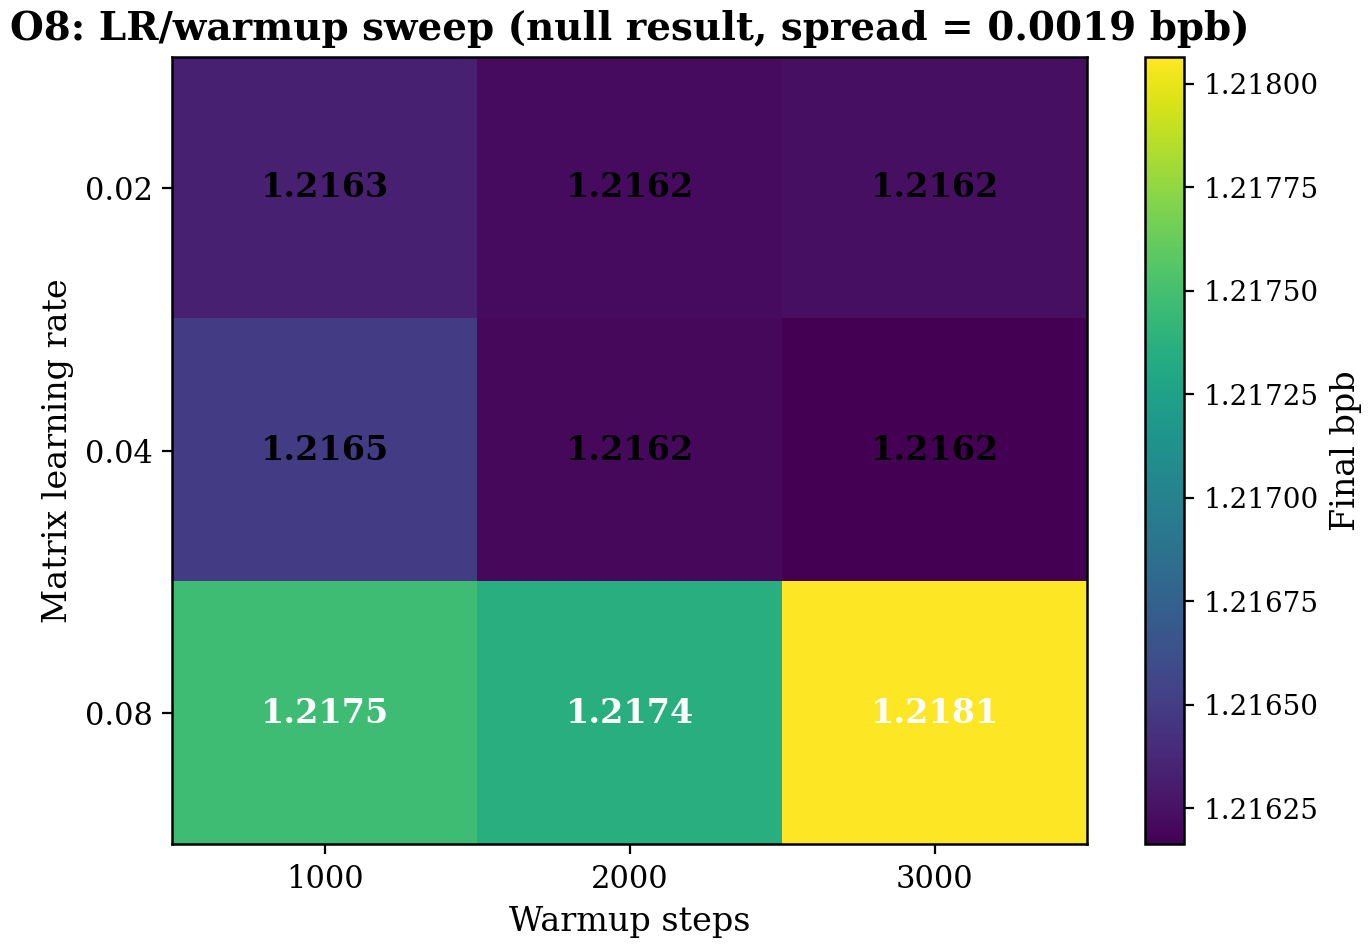
\includegraphics[width=\linewidth]{lr_warmup_heatmap.pdf}
\caption{O8 -- $3{\times}3$ LR/warmup sweep on partial RoPE 9L INT8.
Total spread is 0.0019~bpb, comparable to multi-seed noise on the same
axis.}
\label{fig:o8}
\end{figure}

\subsection{O9 -- Eval protocol}

Bits-per-byte on the FineWeb held-out split is itself a function of
the evaluation protocol. The reference protocol uses non-overlapping
$\ell_{\text{ctx}}{=}1024$ windows. The same INT8+11L weights, evaluated
with a stride-256 sliding window, score \textbf{1.1599~bpb final}, a
0.034~bpb improvement attributable purely to the protocol
(Figure~\ref{fig:o9}). We emphasize that leaderboard-comparable results
must use the non-overlapping protocol; the sliding-window number is a
research-fairness column, not a competitive submission.

\begin{figure}[t]
\centering
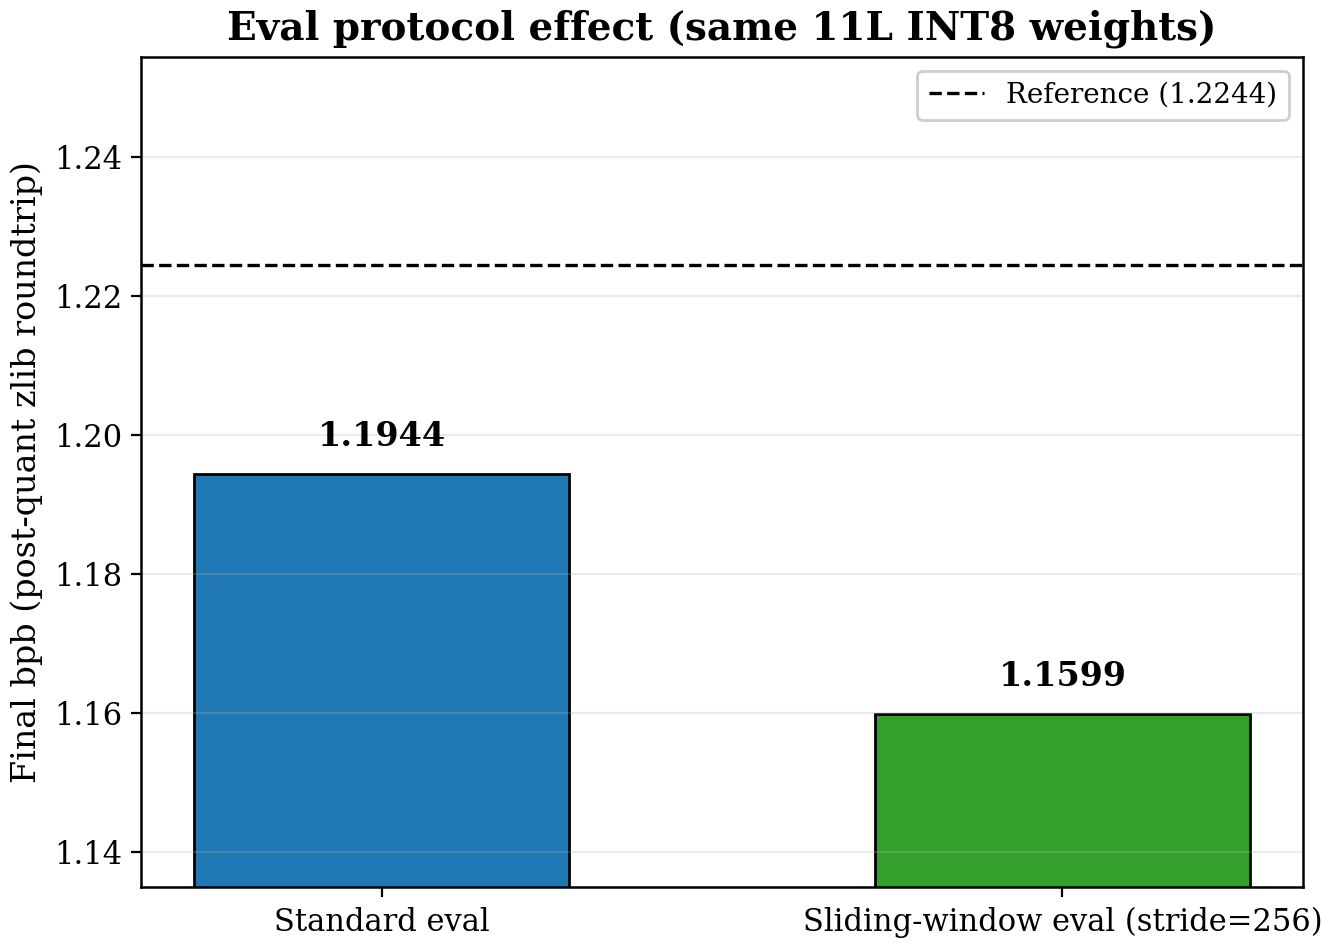
\includegraphics[width=\linewidth]{eval_protocol_bars.pdf}
\caption{O9 -- the same 11L INT8 weights under two eval protocols.
Sliding-window stride-256 systematically reduces bpb by exposing every
token to maximum context.}
\label{fig:o9}
\end{figure}

% ──────────────────────────────────────────────────────────────────────
\section{Multi-Seed Replication}
\label{sec:multiseed}
% ──────────────────────────────────────────────────────────────────────

The proposal's three-seeds-per-condition protocol was executed on the
three surviving in-budget axes: INT8 PTQ (O1), partial RoPE (O2), Muon
optimizer (O3). Standard deviations are tight
(Figure~\ref{fig:multiseed}, Table~\ref{tab:multiseed}), well below
per-axis effect sizes: INT8 $\sigma{=}0.0018$, partial RoPE
$\sigma{=}0.0011$, Muon $\sigma{=}0.0015$. The single-seed claims in
the progress report therefore hold under replication.

\begin{figure}[t]
\centering
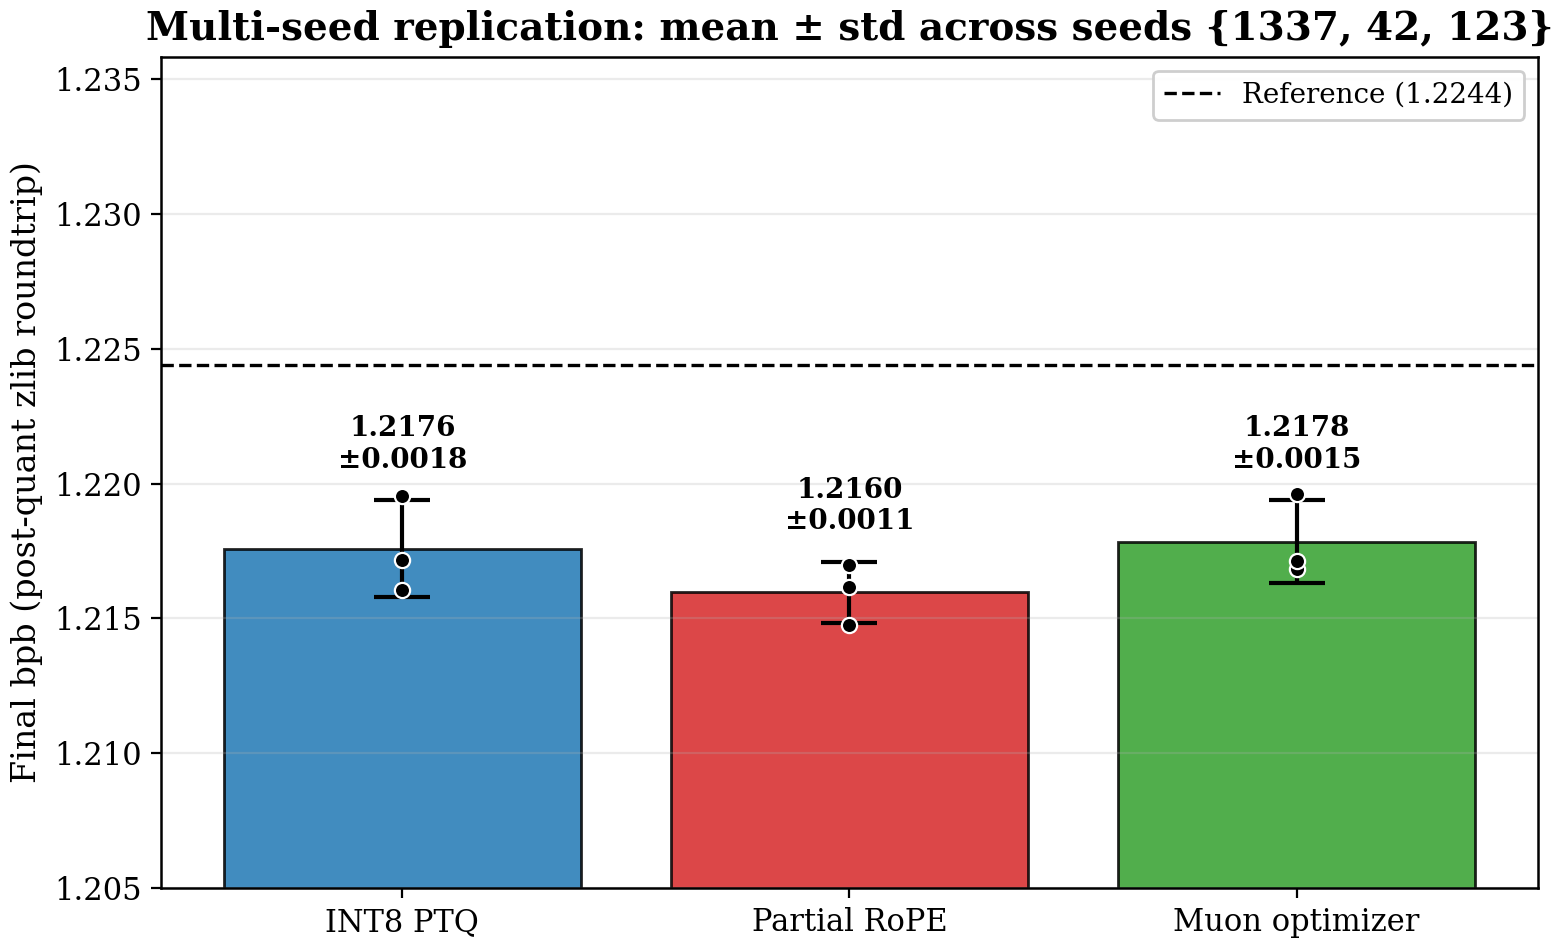
\includegraphics[width=\linewidth]{multiseed_bars.pdf}
\caption{Mean $\pm$ std final bpb across seeds $\{1337, 42, 123\}$ for
the three surviving in-budget axes.}
\label{fig:multiseed}
\end{figure}

\begin{table}[t]
\centering
\caption{Multi-seed final bpb (post-quant zlib roundtrip).
Standard deviations use $n{-}1$ degrees of freedom across $n{=}3$ seeds.}
\label{tab:multiseed}
\small
% auto-generated
\begin{tabular}{@{}lcccc@{}}
\toprule
Condition & Seed 1337 & Seed 42 & Seed 123 & Mean $\pm$ std \\
\midrule
INT8 PTQ & 1.2161 & 1.2172 & 1.2195 & 1.2176 $\pm$ 0.0018 \\
Partial RoPE & 1.2147 & 1.2162 & 1.2170 & 1.2160 $\pm$ 0.0011 \\
Muon optimizer & 1.2168 & 1.2171 & 1.2196 & 1.2178 $\pm$ 0.0015 \\
\bottomrule
\end{tabular}

\end{table}

% ──────────────────────────────────────────────────────────────────────
\section{Pareto Frontier: Headline Finding}
\label{sec:pareto}
% ──────────────────────────────────────────────────────────────────────

Combining all 20{,}000-step runs with their post-quantization artifact
sizes yields the size-quality plane in Figure~\ref{fig:pareto}. The
Pareto frontier (lower-left envelope) has nine points; the four most
informative are labelled.

The frontier exhibits a sharp elbow at $\sim$15.9~MB: below this size,
each MB saved costs roughly 0.02~bpb (steep tradeoff). At and above
this size, the marginal cost flattens substantially -- the in-budget
winner (\texttt{o2\_part\_20k}) and the over-budget winner
(\texttt{stacked\_int8\_safe\_11L\_mlp2\_20k}) sit on the frontier
0.020~bpb apart, separated by 3.3~MB. The MQA + 12L variant
sits very close to the frontier at 19.6~MB / 1.198~bpb but is
dominated by \texttt{stacked\_int8\_safe} on both axes.

The 16~MB reference (red dotted line) crosses the frontier between
two clusters of points. Within the constraint, the partial-RoPE 9L
baseline at 1.2147~bpb is unbeaten by any other 20k-step
configuration we tested. Outside the constraint (16--20~MB), only
INT8 quantization yields configurations on the frontier; INT6,
TurboQuant-INT4, and the structured-weight variants are all dominated.

\begin{figure*}[t]
\centering
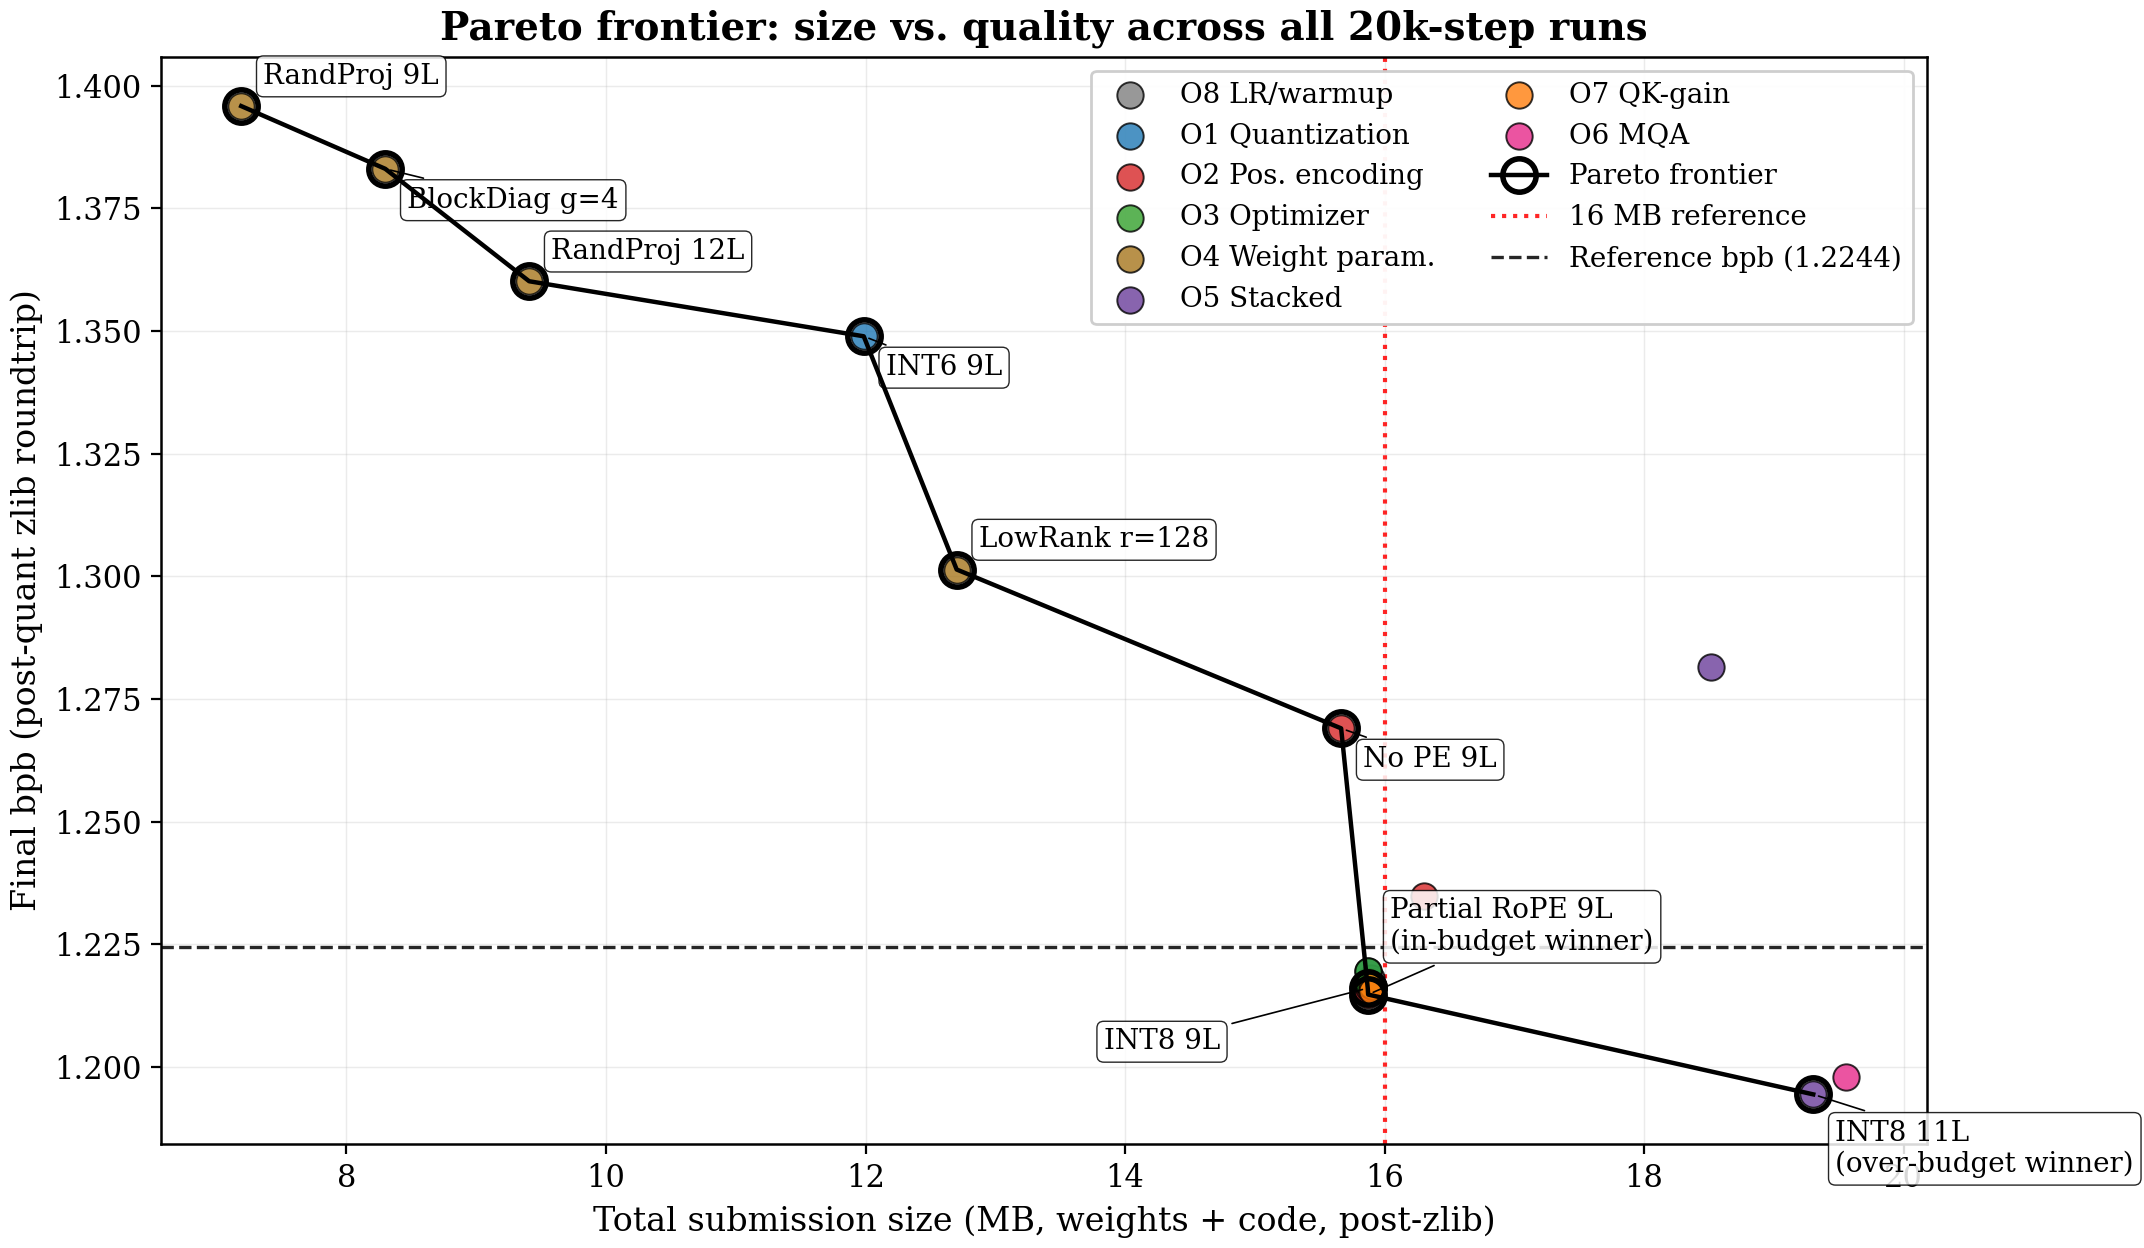
\includegraphics[width=0.92\linewidth]{pareto_frontier.pdf}
\caption{Pareto frontier across all 20{,}000-step runs. X-axis is the
post-quantize, post-zlib total submission size (weights + training
code). Y-axis is the leaderboard-equivalent post-roundtrip bpb. Black
hollow markers and connecting line: frontier. Red dotted line: 16~MB
reference. Black dashed line: 1.2244 reference bpb. The frontier elbow
at 15.9~MB and the 3.3~MB / 0.020~bpb tradeoff above it are the
central quantitative finding of this paper.}
\label{fig:pareto}
\end{figure*}

% ──────────────────────────────────────────────────────────────────────
\section{Aggregated Results}
\label{sec:results}
% ──────────────────────────────────────────────────────────────────────

Table~\ref{tab:results} aggregates every 20{,}000-step run, sorted
within group by post-quantization final bpb. \textsc{Train} is the
in-memory bf16 loss; \textsc{Final} is the post-roundtrip loss;
\textsc{Size} is the total artifact (weights + training code,
post-zlib); $\Delta$ is the gap to the 1.2244 reference; the last
column flags whether the artifact fits the 16~MB reference.

\begin{table*}[t]
\centering
\caption{All 20{,}000-step runs at seed 1337 (where applicable),
grouped by ablation axis. ``Final'' is the post-quant zlib round-trip
bpb. ``Size'' is total submission size (weights + training code,
post-zlib). $\Delta$ is the difference vs.\ the 1.2244 reference; negative is
better.}
\label{tab:results}
\scriptsize
% auto-generated by report/scripts/make_figures.py
\begin{tabular}{@{}llcccc c@{}}
\toprule
Group & Run & Train bpb & Final bpb & Size (MB) & $\Delta$ vs.\ baseline & 16MB \\
\midrule
O10 hpsweep & \texttt{part\_lr040\_wu3000} & 1.2076 & 1.2162 & 15.91 & -0.0082 & OK \\
O10 hpsweep & \texttt{part\_lr040\_wu2000} & 1.2073 & 1.2162 & 15.90 & -0.0082 & OK \\
O10 hpsweep & \texttt{part\_lr020\_wu2000} & 1.2073 & 1.2162 & 15.91 & -0.0082 & OK \\
O10 hpsweep & \texttt{part\_lr020\_wu3000} & 1.2074 & 1.2162 & 15.91 & -0.0082 & OK \\
O10 hpsweep & \texttt{part\_lr020\_wu1000} & 1.2074 & 1.2163 & 15.91 & -0.0081 & OK \\
O10 hpsweep & \texttt{part\_lr040\_wu1000} & 1.2076 & 1.2165 & 15.91 & -0.0079 & OK \\
O10 hpsweep & \texttt{part\_lr080\_wu2000} & 1.2088 & 1.2174 & 15.89 & -0.0070 & OK \\
O10 hpsweep & \texttt{part\_lr080\_wu1000} & 1.2085 & 1.2175 & 15.88 & -0.0069 & OK \\
O10 hpsweep & \texttt{part\_lr080\_wu3000} & 1.2093 & 1.2181 & 15.90 & -0.0063 & OK \\
\midrule
O1 quant & \texttt{int8} & 1.2082 & 1.2161 & 15.87 & -0.0083 & OK \\
O1 quant & \texttt{int8\_20k\_v2} & 1.2082 & 1.2165 & 15.87 & -0.0079 & OK \\
O1 quant & \texttt{int8\_s42} & 1.2095 & 1.2172 & 15.87 & -0.0072 & OK \\
O1 quant & \texttt{int8\_s123} & 1.2110 & 1.2195 & 15.87 & -0.0049 & OK \\
O1 quant & \texttt{int6} & 1.2083 & 1.3489 & 11.99 & +0.1245 & OK \\
\midrule
O2 posenc & \texttt{part} & 1.2071 & 1.2147 & 15.87 & -0.0097 & OK \\
O2 posenc & \texttt{part\_20k\_v2} & 1.2068 & 1.2153 & 15.87 & -0.0091 & OK \\
O2 posenc & \texttt{part\_s42} & 1.2078 & 1.2162 & 15.88 & -0.0082 & OK \\
O2 posenc & \texttt{part\_s123} & 1.2084 & 1.2170 & 15.87 & -0.0074 & OK \\
O2 posenc & \texttt{rope} & 1.2085 & 1.2174 & 15.88 & -0.0070 & OK \\
O2 posenc & \texttt{learn} & 1.2244 & 1.2349 & 16.30 & +0.0105 & OVER \\
O2 posenc & \texttt{none} & 1.2589 & 1.2690 & 15.67 & +0.0446 & OK \\
\midrule
O3 optim & \texttt{muon} & 1.2089 & 1.2168 & 15.88 & -0.0076 & OK \\
O3 optim & \texttt{muon\_s42} & 1.2085 & 1.2171 & 15.87 & -0.0073 & OK \\
O3 optim & \texttt{muon\_s123} & 1.2117 & 1.2196 & 15.87 & -0.0048 & OK \\
\midrule
O4 weightparam & \texttt{lr128} & 1.2915 & 1.3014 & 12.70 & +0.0770 & OK \\
O4 weightparam & \texttt{rp128\_12L} & 1.3472 & 1.3601 & 9.41 & +0.1357 & OK \\
O4 weightparam & \texttt{bd4} & 1.3700 & 1.3830 & 8.30 & +0.1586 & OK \\
O4 weightparam & \texttt{rp128} & 1.3838 & 1.3958 & 7.19 & +0.1714 & OK \\
\midrule
O5 stacked & \texttt{stacked\_int8\_safe\_11L\_mlp2\_slide256} & 1.1524 & 1.1599 & 19.30 & -0.0645 & OVER \\
O5 stacked & \texttt{stacked\_int8\_safe\_11L\_mlp2} & 1.1869 & 1.1944 & 19.30 & -0.0300 & OVER \\
O5 stacked & \texttt{stacked\_v1\_pr\_int6\_11L\_mlp3\_20k\_v2} & 1.1618 & 1.2801 & 18.52 & +0.0557 & OVER \\
O5 stacked & \texttt{stacked\_v1\_pr\_int6\_11L\_mlp3} & 1.1614 & 1.2816 & 18.52 & +0.0572 & OVER \\
O5 stacked & \texttt{stacked\_tq4\_big\_11L\_mlp3\_20k\_v2} & 1.1612 & 3.5991 & 12.91 & +2.3747 & OK \\
\midrule
O8 qkgain & \texttt{qk3p0} & 1.2065 & 1.2154 & 15.91 & -0.0090 & OK \\
O8 qkgain & \texttt{qk5p0} & 1.2083 & 1.2165 & 15.91 & -0.0079 & OK \\
\midrule
O9 attn & \texttt{mqa\_12L\_mlp2\_int8} & 1.1909 & 1.1980 & 19.56 & -0.0264 & OVER \\
\bottomrule
\end{tabular}

\end{table*}

% ──────────────────────────────────────────────────────────────────────
\section{Discussion}
% ──────────────────────────────────────────────────────────────────────

\subsection{Key findings}

\begin{enumerate}[leftmargin=*]
    \item \textbf{Sub-INT8 weight quantization is fragile at this scale.}
          INT6 QAT loses 0.14~bpb under round-trip; TurboQuant-INT4
          loses 2.44~bpb, sixteen times worse. QAT does not close the
          INT6 gap; random rotation does not save INT4. The problem is
          the post-training scalar quantizer applied to weights at
          this distribution scale, not the training recipe.
    \item \textbf{Partial RoPE is the strongest in-budget modification.}
          1.2147~bpb final beats every other single-axis condition we
          tested at 15.87~MB. Multi-seed $\sigma{=}0.0011$.
    \item \textbf{Muon is load-bearing, not marginal.} AdamW and
          Adafactor lose more than 0.2~bpb. Multi-seed $\sigma{=}0.0015$.
    \item \textbf{Capacity expansion is real and recoverable -- if and
          only if the quantizer is INT8.} INT8 + 11L + MLP=2 at
          19.30~MB delivers 1.1944~bpb. The same expansion under INT6
          forfeits the gain; under TurboQuant-INT4 collapses entirely.
    \item \textbf{Multi-Query Attention enables 12-layer depth.}
          1.1980~bpb final at 19.56~MB, on the same arm of the
          frontier as the INT8+11L winner.
    \item \textbf{Structured weight factorizations do not help.} O4 is
          a falsified hypothesis.
    \item \textbf{Per-condition LR/warmup tuning is also a null effect.}
          The 3$\times$3 sweep is flat to within multi-seed noise.
    \item \textbf{Size-quality is a smooth Pareto frontier with a sharp
          elbow at $\sim$16~MB.} The 16~MB constraint is not a natural
          break; reading the data as a Pareto curve recovers a clean
          monotone tradeoff and surfaces multiple legitimate frontier
          configurations across 7--20~MB.
\end{enumerate}

\subsection{Limitations}

The 20{,}000-step training horizon is a fixed slice; we do not test
whether longer training inverts the architectural ranking, although
prior scaling-law work suggests it does not at this parameter
count~\cite{kaplan2020}. We do not retest TurboQuant on activations
where it was originally validated~\cite{turboquant2024}; our negative
result applies specifically to weights at this scale. Multi-seed
replication was performed only on the three surviving in-budget axes,
not on the over-budget winners.

\subsection{Demonstration: in-browser interpretability tool}

The 16~MB winner is small enough to ship as a static web page. We
packaged the in-budget winner as a client-side ONNX
Runtime~Web~\cite{onnxruntimeweb} demo: a static HTML file that
accepts a user-typed prefix and renders, in real time, the top-$k$
next-token distribution with probability bars, the per-head attention
heatmap over input tokens, and the L2 norm of each layer's hidden
state. Inference runs entirely in the browser; no server is involved.
The choice of an interpretability surface (rather than a generic
autocomplete UI) is deliberate -- the model's small size makes every
internal state cheap to render live, which would be infeasible at
conventional language-model scale.

% ──────────────────────────────────────────────────────────────────────
\begin{thebibliography}{99}

\bibitem{paramgolf2026}
OpenAI.
\newblock OpenAI Model Craft: Parameter Golf Challenge, 2026.
\newblock \url{https://github.com/openai/parameter-golf}

\bibitem{fineweb2024}
G. Penedo et al.
\newblock {The FineWeb Datasets: Decanting the Web for the Finest Text
Data at Scale}.
\newblock arXiv preprint arXiv:2406.17557, 2024.

\bibitem{scalingprecision}
K. Kumar et al.
\newblock {Scaling Laws for Precision}.
\newblock ICLR, 2025. arXiv:2403.08540.

\bibitem{rope}
J. Su et al.
\newblock {RoFormer: Enhanced Transformer with Rotary Position Embedding}.
\newblock arXiv preprint arXiv:2104.09864, 2021.

\bibitem{muon2024}
K. Jordan et al.
\newblock {Muon: An Optimizer for the Hidden Layers of Neural Networks}.
\newblock Technical report, 2024.

\bibitem{turboquant2024}
A. Zandieh et al.
\newblock {TurboQuant: Online Vector Quantization with Near-Optimal
Distortion Rate}.
\newblock arXiv preprint, 2024.

\bibitem{mqa2019}
N. Shazeer.
\newblock {Fast Transformer Decoding: One Write-Head is All You Need}.
\newblock arXiv preprint arXiv:1911.02150, 2019.

\bibitem{kaplan2020}
J. Kaplan et al.
\newblock {Scaling Laws for Neural Language Models}.
\newblock arXiv preprint arXiv:2001.08361, 2020.

\bibitem{hoffmann2022}
J. Hoffmann et al.
\newblock {Training Compute-Optimal Large Language Models}.
\newblock arXiv preprint arXiv:2203.15556, 2022.

\bibitem{onnxruntimeweb}
Microsoft.
\newblock {ONNX Runtime Web -- Run ONNX models in the browser}.
\newblock \url{https://onnxruntime.ai/docs/tutorials/web/}

\end{thebibliography}

\end{document}
